%%%%%%%%%%%%%%%%%%%%%%%%%%%%%%%%%%%%%%
  %%%%%%%%%%%%%%%%%%%%%%%%%%%%%%%%%%%%%%
  % Do not edit the TeX file your work
% will be overwritten.  Edit the RnW
% file instead.
%%%%%%%%%%%%%%%%%%%%%%%%%%%%%%%%%%%%%%
  %%%%%%%%%%%%%%%%%%%%%%%%%%%%%%%%%%%%%%
  


We demonstrate the local sensitivity computations on a 
Gaussian mixture model (GMM) of the iris dataset. 
The model and variational approximation were detailed in 
\exref{iris_bnp_process,iris_var_distr}, respectively. 
\figref{iris_fit} shows the GMM fit at $\alpha = 6$. 
The data consists of three species of iris, and
the BNP model correspondingly identifies three dominant clusters. 


\begin{knitrout}
\definecolor{shadecolor}{rgb}{0.969, 0.969, 0.969}\color{fgcolor}\begin{figure}[!h]

{\centering 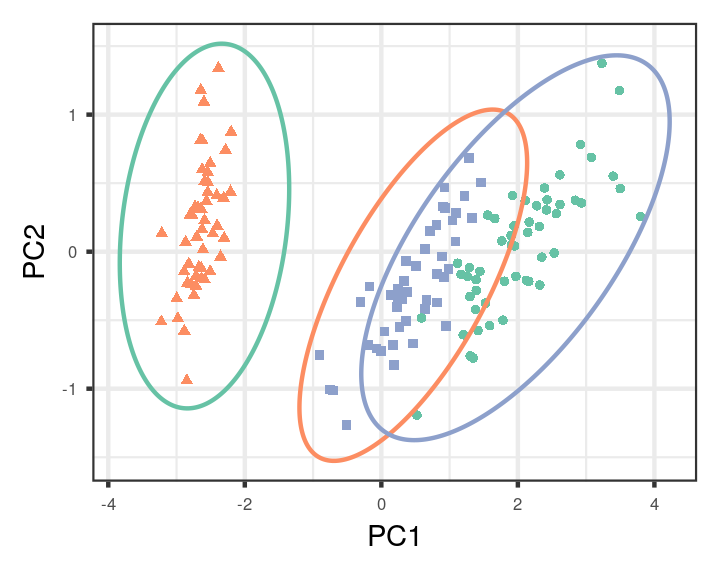
\includegraphics[width=0.588\linewidth,height=0.470\linewidth]{figure/iris_fit-1} 

}

\caption[The iris data in principal component space and 
                      GMM fit at $\alpha = 6$]{The iris data in principal component space and 
                      GMM fit at $\alpha = 6$. 
                      Colors denote inferred memberships and
                      ellipses are estimated covariances. }\label{fig:iris_fit}
\end{figure}


\end{knitrout}

We wish to evaluate the sensitivity of the expected number of clusters to the 
stick-breaking distribution. 
Define the expected number of \textit{in-sample} clusters as
\begin{align*}
\gclusters(\eta) &= \expect{\q(\z\vert\eta)}{\sum_{k=1}^\kmax \ind{ \sum_{n=1}^{N}
\z_{\n\k} > 0}} \\ 
&= \sum_{k=1}^\kmax \left(1 -  \prod_{n=1}^N
\left(1 - \expect{\q(\z_{nk}\vert\eta)}{\z_{nk}}\right)\right).
\end{align*}
%
The in-sample quantity $\gclusters$ is an estimate for 
the number of species present in the observed iris dataset. 
Alternatively, we can define a {\itshape posterior predictive} quantity, 
which is an estimate of the number of species one would expect to see 
should a new iris dataset of size $N$ be collected.
Define the posterior predictive number of clusters as 
\begin{align*}
\gclusterspred(\eta) = \expect{\q(\nu\vert\eta)}{\sum_{k}^\kmax\left(1 -
(1 - \pi_k)^N\right)},
\end{align*}
where recall that $\pi_k$ are the mixture weights computed from the stick-lengths, $\pi_\k = \nuk \prod_{\k' < \k} (1 - \nu_{\k'})$.

We first consider the sensitivity of these posterior quantities 
$\gclusters$ and $\gclusterspred$ 
to the prior parameter $\alpha$. 
\figref{beta_priors} displays the probability density functions 
$\pstick(\nuk \vert \alpha) = \betadist{\nuk \vert 1, \alpha}$ 
for a range of $\alpha$. 

We first fit the model at $\alpha = 6$. 
Subsequent refits at $\alpha\not=6$ used the fit at $\alpha = 6$ as an initialization. 
As $\alpha$ increases, the expected number of clusters increases (\figref{iris_alpha_sens}). 
The expected number of in-sample clusters is relatively insensitive to changes in the $\alpha$ parameter. 
As $\alpha$ varies from $\alpha = 1, ..., 16$, the $g_{\text{n.cl.}}$ varies 
only from 3 to 3.4 (recall that the true number of iris species is three). 
On the other hand the posterior preditive quantitiy is sensitive to changes in $\alpha$. Over the same range of $\alpha$, $g_{\text{n.cl.pred}}$ varies from 
3.6 to 8.1. 

The linear approximation captures the changes in both the in-sample and predictive number of clusters. 
We computed the linear approximation at $\alpha = 6$. 
Forming the linear approximation, which requires inverting the Hessian matrix, required TODO seconds. 
Subsequent evaluations of $\etalin(\alpha)$ for any $\alpha$ requires only a vector-scalar multiplication and vector-vector addition. 
Thus, after forming the linear approximation at $\alpha = 6$,
using the approximation to form the path of $g$ as $\alpha$ varies in
\figref{iris_alpha_sens} took only TODO seconds. 
On the other hand, to form the path of $g$ by refitting at each $\alpha$ in 
\figref{iris_alpha_sens} took TODO seconds in total, with a median refit time of TODO. 




\begin{knitrout}
\definecolor{shadecolor}{rgb}{0.969, 0.969, 0.969}\color{fgcolor}\begin{figure}[!h]

{\centering 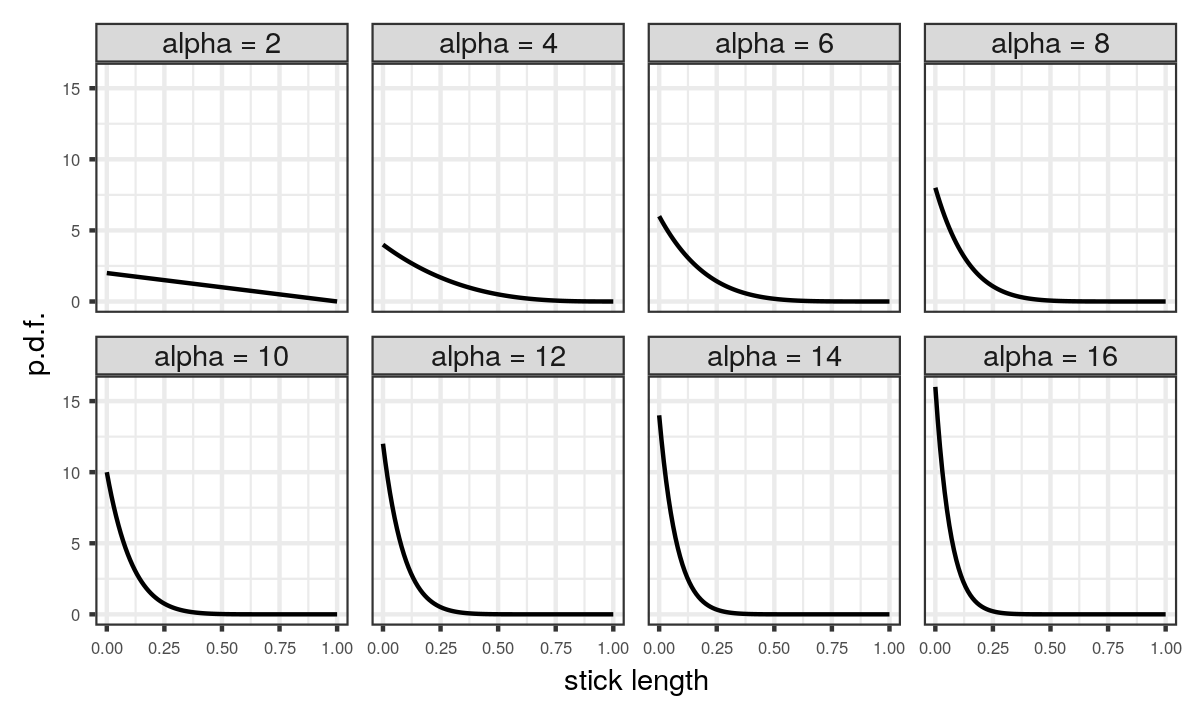
\includegraphics[width=0.980\linewidth,height=0.588\linewidth]{figure/beta_priors-1} 

}

\caption[Probability density functions of $\text{Beta}(1, \alpha)$ distributions, for various $\alpha$]{Probability density functions of $\text{Beta}(1, \alpha)$ distributions, for various $\alpha$. }\label{fig:beta_priors}
\end{figure}


\end{knitrout}


\begin{knitrout}
\definecolor{shadecolor}{rgb}{0.969, 0.969, 0.969}\color{fgcolor}\begin{figure}[!h]

{\centering 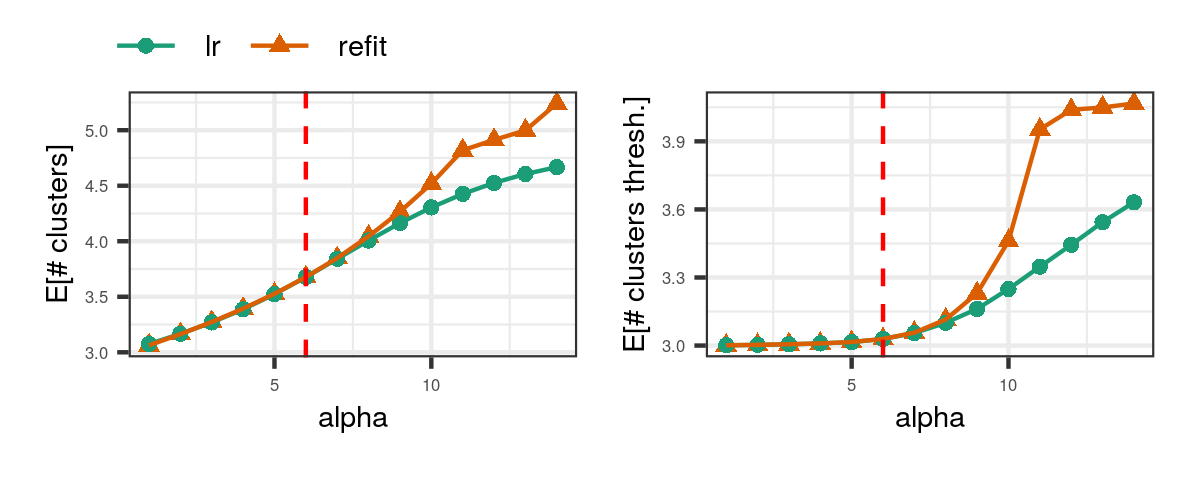
\includegraphics[width=0.980\linewidth,height=0.392\linewidth]{figure/iris_alpha_sens-1} 

}

\caption[The expected number of clusters as $\alpha$ varies in the 
the BNP-GMM fit of the iris data]{The expected number of clusters as $\alpha$ varies in the 
the BNP-GMM fit of the iris data. 
On the left is the sensitivity of the in-sample quantity.  
On the right is the the predictive quantity. 
We compute the linear approximation at $\alpha=6$ and
extrapolate the expected number of clusters using the
linear approximation (green).
We compare against the expected number of clusters obtained by refitting the model at each $\alpha$ (orange). }\label{fig:iris_alpha_sens}
\end{figure}


\end{knitrout}



\begin{knitrout}
\definecolor{shadecolor}{rgb}{0.969, 0.969, 0.969}\color{fgcolor}\begin{figure}[!h]

{\centering 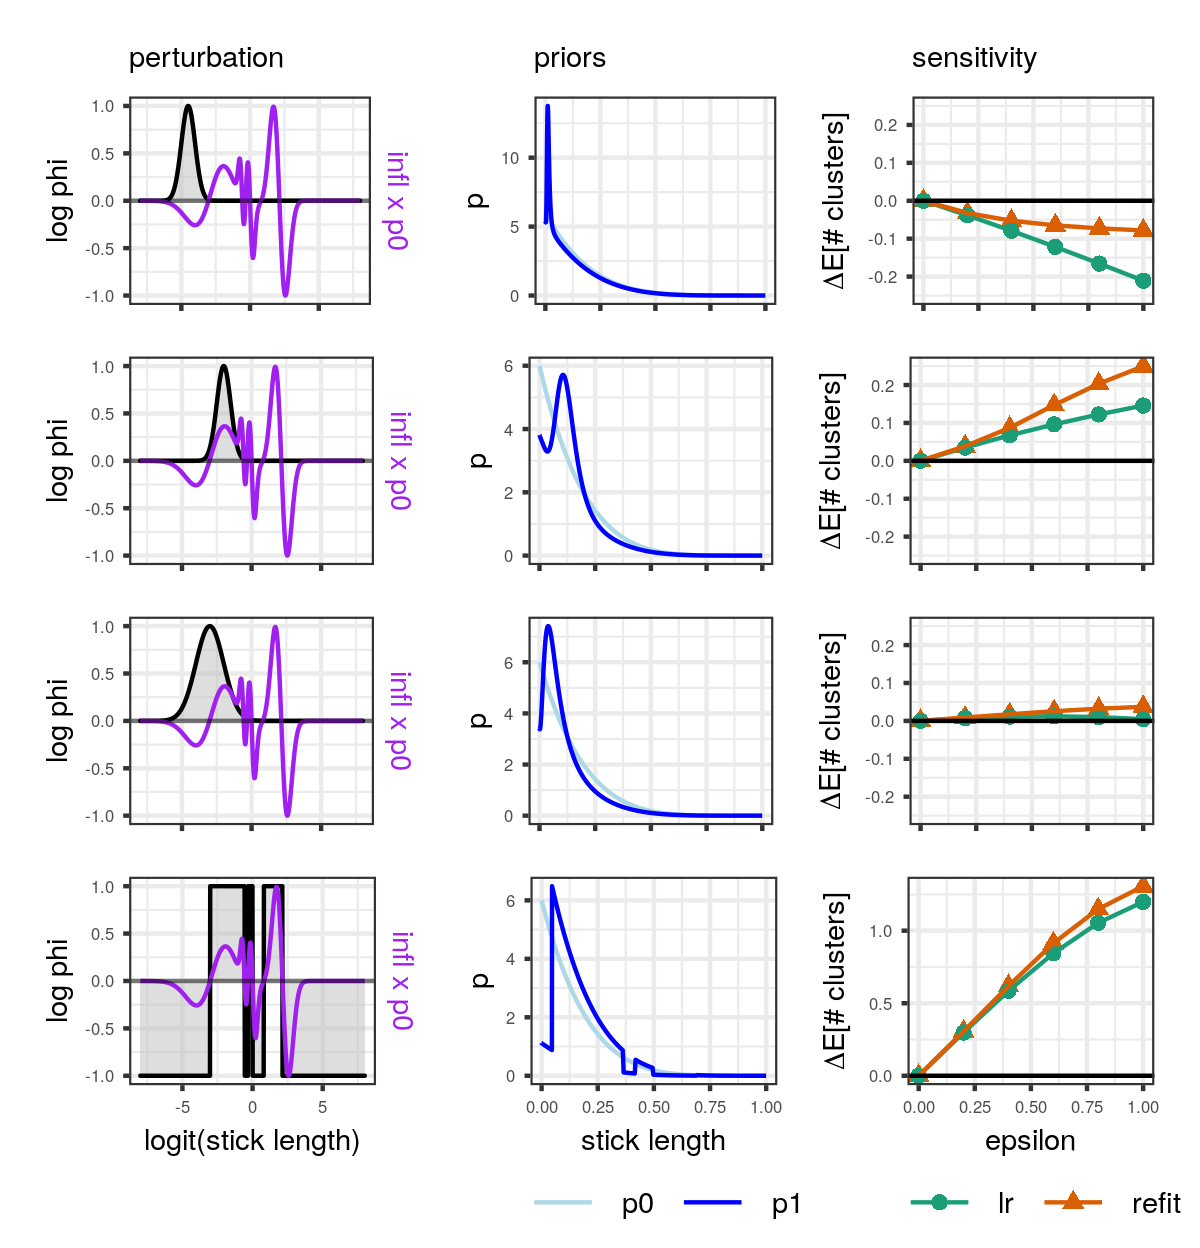
\includegraphics[width=0.980\linewidth,height=1.019\linewidth]{figure/iris_fsens-1} 

}

\caption{Sensitivity of
        the expected number of in-sample clusters in the iris dataset
        to four multiplicative perturbations with 
        $L_{\infty}$-norm equal to one. 
        (Left) The log multiplicative perturbation $\log\phi$ in grey.        
        In purple is the prior-weighted influence function, scaled to also have 
        unit $L_{\infty}$-norm. 
        (Middle) The original prior density $p_0$ and 
        the perturbed prior density $p_1 = p_0\times \phi$. 
        (Right) The effect of the perturbation 
        on the change in expected number of clusters as a function of $\epsilon$. }\label{fig:iris_fsens}
\end{figure}


\end{knitrout}


\begin{table}[tb]
\centering
\caption{Compute time of results on the iris dataset. }
\begin{tabular}{|r|r|}
    \hline 
    & time (seconds) \\ 
    \hline 
    Initial fit & 0.96 \\
    \hline 
    Hessian solve for $\alpha$ sensitivity & 
        0.021\\
    Linear approx. $\eta^{lin}(\alpha)$ for $\alpha = 1, ... , 16$ & 
        0.018\\
    Refits $\eta(\alpha)$ for $\alpha = 1, ... , 16$ & 
        9.6\\
    \hline 
    Hessian solve for worst-case $\phi$ & 
        0.021\\
    Linear approx. $\eta^{lin}(\epsilon)|_{\epsilon = 1}$
    for worst-case $\phi$ & 
        0.0011\\
    Refit $\eta(\epsilon)|_{\epsilon = 1}$ for worst-case $\phi$ & 
        0.72\\ 
    \hline 
    The influence function & 0.1\\ \hline
\end{tabular}
\end{table}

